\section {度量衡单位及转换}

-
    \begin{center}
        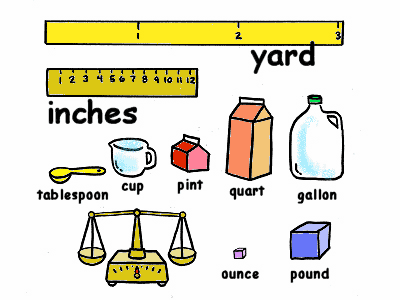
\includegraphics[scale=0.7] {units.png}
    \end{center}

\subsection {单位系统}

        单位系指给定的某一基础物理量,单位的给定皆属人为。常伴随着某种表示法,例如米、秒、公斤等,以方便人们在沟通某一量时有共通的概念。

        计量单位或计算单位为单位的具体统称,为人类计算一个数额的方法。例如,在数字中,单位一般为“1”;在计算长度的时候,单位可以是“纳米”、“毫米”、“厘米(或作厘米)”、“分米”、“米”、“千米”、“光年”等;在计算时间的时候,单位可以是“微秒”、“秒”、“分钟”、“时”、“日”、“星期”、“月”、“年”、“世纪”等。

    \subsubsection {单位制}

        由选定的基本单位和它们的导出单位组成的一系列量度单位的总称。

    \subsubsection {基本单位}

        各种物理量都有它们的量度单位,并以选定的物质在规定条件下所显示的数量作为基本量度单位的标准,在不同时期和不同的学科中,基本量的选择何以不同。如物理学上以时间、长度、质量、温度、电流强度、发光强度、物质的量这7个物理单位为基本量,它们的单位依次为:秒、米、千克、开尔文、安培、坎德拉、摩尔。 还有一种说法不包含电流强度,而是磁力强度,单位是特兹拉。

    \subsubsection {导出单位}

        由于基本量根据有关公式推导出来的其他量,叫做导出量。导出量的单位叫做导出单位。如速度的单位是由长度和时间单位组成的用“m/s”表示。

    \subsubsection {组合单位}

        由其他量的单位组合而成的单位叫做组合单位。如压强的单位(Pa)可以用力的单位(N)和面积的单位(m2)组成,即:N/m2。



\subsection {单位转换}

    每个物料有一个基本的单位称为“主单位”。比如桌子的单位一定是“张”,而不是“公斤”。但每张具体的桌子都有一个确定的质量,描述这个质量的单位被称为“辅助单位”。

    不同的物料可以有相同的主单位,但换算为辅助单位所使用的比例通常是不同的。

    在本系统中,每个物料除了有一个确定的主单位外,还可以设置若干个辅助单位,并通过单位换算表来确定物料在辅助单位下的数量。

    在进行单位换算时,所有数量将首先换算为标准量纲下的单位,比如毫米将先换算为0.001米,千克将先换算为1000克,然后再进行不同单位类型之间的换算。

    为了减轻资料的录入工作,单位换算表是可以复用的,这就是说在编辑物料信息时,可以为每一个物料创建一个专用的换算表,也可以指定一个已经存在的换算表。
